\documentclass[../main.tex]{subfiles}

\begin{document}
\chapter{Physically Based Rendering}

\section{Wstęp}

W początkach lat 2000 ze względu na ograniczenia techniczne najpopularniejszym
modelem wykorzystywanym w grach był model Blinna-Phonga, który nie wymagał
dużej mocy obliczeniowej do oświetlenia nawet złożonych scen. Model ten
korzystał z kilku podstawowych zasad geometrycznych do opisu oświetlenia.
Równanie Blinna-Phonga opisane jest prostym równaniem:

\begin{gather*}
  L_o(p) = k_e + k_a I_a +
    \sum_{m \in L} \left( {
      k_d L_m \max\left({ \omega_m \cdot n, 0 }\right) +
      k_s L_m (n \cdot h)^{\alpha}
    } \right) \\
    h = \frac{\omega_o+\omega_m}{||\omega_o+\omega_m||}
\end{gather*}

W równaniu pojawiają się pewne dobrane przez artystę stałe materiałowe
opisujące dany punkt na powierzchni, a mianowicie:

\begin{itemize}
\item $k_e$ - współczynnik będący ilością światła wyemitowanego w punkcie,
  opisuje on ilość wysłanej energii z punktu, wartość ta nie jest zależna
  od żadnego innego czynnika, współczynnik ten może pomóc w modelowaniu
  żarzącego się metalu, diód na urządzeniach elektronicznych itp.

\item $k_a$ - współczynnik odbicia światła otoczenia określa jaka część swiatła
  pochodzącego z otoczenia jest odbita do obserwatora, w starszych grach źródłem
  światła z otoczenia były tzw. mapy środowiskowe (ang. \textit{environment
  maps});

\item $k_d$ - współczynnik odbicia światła rozproszonego określa ilość światła
  odbitego równomiernie w każdym kierunku (ilość odebranego światła przez
  obserwatora jest niezależna od kąta obserwacji), wartość ta opisuje generalnie
  kolor materiału

\item $k_s$ - współczynnik odbicia światła lustrzanego, opisuje on kolor światła
  odbitego od powierzchni, decyduje on o kolorze refleksów

\end{itemize}

Jak widać, powyższe stałe są tak naprawde kolorami różnych typów interakcji
wiązki światła z pewnych źródeł z powierzchnią. Kolor odbicia zależy w bardzo
dużym stopniu od artysty i jego wyobrażenia o zachowaniu światła w danym
środowisku, nie wynika on jasno z właściwości materiału, lecz zwykłego domysłu
jak poszukiwany materiał się zachowa i w jaki sposób będzie połyskiwał.

Doprowadza to sytuacji, w których obiekt, dla którego stworzone są tekstury
może wyglądać bardzo dobrze w jednym otoczeniu, by w drugim wyglądać
nienaturalnie: zaprojektowany model wraz z mapami może bardzo dobrze
prezentować się na zewnątrz pośród trawy, lecz w słabo oświetlonej jaskini nie
będzie sprawiał wrażenia naturalnego, wrażenia istnienia w i razem z tym
miejscem. Zatem jednym z głównych problemów prostych modeli oświetlenia jest
to, że bardzo często nie wyglądają one naturalnie w różnych warunkach
oświetlenia.

Podejście PBR wychodzi naprzeciw oczekiwaniom i rozwiązuje ten problem
zmieniając podejście do tworzenia sceny. Artyści zamiast próbować dobrać
współczynniki tak, aby uzyskać pewien efekt wizualny zgodny z naturalnym
używają współczynników opisujących materię. W ten sposób nie opierają się oni
na niedoskonałych domysłach i zmyśle artystycznym, przekładając
odpowiedzialność za poprawny wygląd w dowolnej scenie na modele matematyczne.
Opis staje się niezależny od oświetlenia co jest dużą oszczędnością w procesie
produkcyjnym.

Kolejnym problemem prostych modeli oświetlenia jest brak zachowania
podstawowych zasad fizycznych, w tym zasady zachowania energii. W szczególności
równania Blinna-Phonga ze względu na prostą strukturę nie umożliwiają na
precyzyjną kontrolę jaka część energii zostaje rozproszona, a jaka odbita. Bez
ingerencji artysty (lub programisty) często dochodzi do sytuacji w której
refleksy są nienaturalne, prześwietlone w wyniku wygenerowania energii przez
dany obszar powierzchni. Jest to skutkiem braku ograniczenia suma energii
wychodzącej do całkowitej energii przychodzącej (ignorując zjawisko emisji
światła przez rozżarzony metal, żarówki i inne). W obszarze w którym więcej
światła ulega odbiciu, mniej światła może może ulec rozproszeniu.

Model Blinna-Phonga również nie jest w stanie realistycznie obsłużyć wielu
typów materiałów, w tym metali. Metale cechują się pełną absorpcją światła
załamanego. W takim przypadku dokładny model zachowania światła odbitego ma
bardzo duże znaczenie dla końcowego wyglądu sceny.

Minusem bardziej zaawansowanych modeli oświetlenia jest ich zapotrzebowanie na
moc obliczeniową. Przeprowadzenie wymaganych obliczeń wymaga kilkukrotnie
większej ilości operacji, modele opisane w tym rozdziale w większości powstały
w latach 80, jednak ich użycie nie było możliwe przez wiele lat w aplikacjach
czasu rzeczywistego. Obecny sprzet jednak pozwala nam na zastosowanie ich bez
dużego kosztu wydajności.

\section{Analiza geometryczna wiązki światła}

Rozważania na temat modelu zgodnego z fizyką rozpoczniemy od analizy natury
wiązki światła. Zrozumienie sposobu w jaki wiązka światła zachowuje się po
zderzeniu z idealnie równą powierzchnią jest fundamentem całej dziedziny metod
poprawnych fizycznie.

Światło jest falą o pewnej długości $\lambda$, fale o różnej długości tworzą
wiązkę światła. Widmo optyczne (spektrum) jest rozkładem długości fal danej
wiązki. Naturalne wiązki światła posiadają nieskończoną ilość długości fal,
jednak w grafice komputerowej stosuje się przybliżenie trzema długościami fal
które odpowiadają trzem kolorom: czerwonemu (ang. red, R), zielonemu (ang.
green, G) i niebieskiemu (ang. blue, B).

\begin{figure}[ht]
  \missingfigure{Ilustracja spektrum światła i przybliżenie RGB}
\end{figure}

Światło może poruszać się w różnego rodzaju ośrodkach w powietrzu, soku, mleku,
skórze czy plastiku. Sposób poruszania się w takim ośrodku zależy od kilku
czynników.

Najprostszym ośrodkiem jest medium jednorodne, które ma jednolitą strukturę
wewnętrzną na skutek czego prędkość światła w każdym punkcie i w każdym
kierunku jest jednakowa. W takim przypadku światło w ośrodku porusza się w
linii prostej. Najlepszym przykładem ośrodka tego typu jest próżnia. Mimo braku
zmiany kierunku w niektórych ośrodkach które możemy uważać za jednorodne
następuje utrata energii na skutek absorpcji wynikającej ze zderzeń z atomami
materii np. w wodzie.

Ośrodkiem niejednorodnym nazywamy ośrodek o niejednorodnej strukturze
wewenętrznej, w którym prędkość światła jest zależna od kierunku lub badanego
miejsca. Ze względu na to, światło jest załamywane i w mocno niejednorodnych
objawia się to  wymieszaniem światła (światło biegnie w losowych kierunkach).

Wiązka światła podczas zderzenia z powierzchnią (dokładniej, przy przejściu z
jednego ośrodka do drugiego) rozdziela się na dwie części: część odbitą od
powierzchni oraz załamaną - część ze zmienionym kierunkiem ale wchodzącym do
nowego ośrodka.

Część energii, która została uległa refrakcji wchodzi wgłąb obiektu, gdzie
zachodzą kolejne kolizje z atomami materii, przez co znów dochodzi do
powyższego zjawiska, tym razem we wnętrzu obiektu. Część tego światła może
wydostać się z obiektu i dotrzeć do obserwatora, pozostała część zostanie
pochłonięta i zamieniona na inne rodzaje energii np. ciepło.

Zauważmy, że w przypadku braku emisji energii energia która dociera do
obserwatora musi być mniejsza lub równa energii wiązki światła - ta właściwość
jest jednym z filarów podejścia fizycznie poprawnego. W przypadku metali
jednak, światło które trafi do wnętrza takiego obiektu zostaje bardzo szybko
zaabsorbowane. Energia światła zostaje zamieniona na inny jej rodzaj przez
wolne elektrony w strukturze metalu.

W modelach matematycznych wymienionych w tej pracy zakładamy, że ponowne
wyjście energii która była poddana refrakcji następuje w tym samym punkcie, w
którym promień zderzył się z powierzchnią (rys. \ref{fig:ReflectionRefraction}).

% Rysunek odbicia z płaską powierzchnią (model uproszczony)
\begin{figure}[h]
  \centering
  \begin{tikzpicture}
    %\draw[help lines] (-5,-1) grid (5,5);
    \draw [thick] (-5.0,0.0) -- (5.0,0.0);

    % Specular
    \foreach \i in {0,...,5} {
      \pgfmathtruncatemacro{\angle}{90+30+(\i / 5) * 30};
      \draw [-Triangle, blue] (0,0) -- ( {3*cos(\angle)}, {3*sin(\angle)} );
    }

    % Diffuse
    \foreach \i in {1,...,15} {
      \pgfmathtruncatemacro{\angle}{(\i / 16) * 180};
      \draw [-Triangle, gray] (0,0) -- ( {2*cos(\angle)}, {2*sin(\angle)} );
    }

    \draw [fill] (2,2) circle [radius=0.05] node [above] {\Large\faLightbulbO};
    \draw [-{Triangle[scale=2]}] (2,2) -- (0,0);
  \end{tikzpicture}
  \caption{Przybliżony model interakcji wiązki światła z powierzchnią}
  \label{fig:ReflectionRefraction}
\end{figure}

Istnieją techniki które biorą pod uwagę możliwość ucieczki energii w innym
miejscu, ale skomplikowałyby one rozważania na których skupia się ta praca.
Techniki takie są wymagane do uzyskania realistycznych obrazów w którym pojawia
się skóra, work i inne materiały w których rozproszenie podpowierzchniowe
jest widoczne.

\begin{figure}[ht]
  \centering
  \begin{tikzpicture}
    %\draw[help lines] (-5,-1) grid (5,5);

		\coordinate (left) at (-3,0);
		\coordinate (right) at (3,0);
    \draw [ultra thick] (left) -- (right);

		\coordinate (normal) at (0,3);
		\coordinate (invnormal) at (0,-3);

    \draw  [-{Triangle[scale=2]}] (invnormal) -- (normal) node [above] {$N$};

		\coordinate (orig) at (0,0);
		\coordinate (light) at (45:3);
		\coordinate (reflection) at (135:3);
		\coordinate (refraction) at (205:3);

    \draw  [-{Triangle[scale=2]}] (orig) -- (reflection)
      node [midway, above] {$r$};
    \draw  [-{Triangle[scale=2]}] (orig) -- (refraction)
      node [midway, above] {$t$};
    \draw  [-{Triangle[scale=2]}] (light) -- (orig);

    \draw pic[draw=black, <->, "$\alpha_i$", angle eccentricity=1.5]
			{angle = light--orig--normal};

    \draw pic[draw=black, <->, "$\alpha_r$", angle eccentricity=1.5]
			{angle = normal--orig--reflection};

    \draw pic[draw=black, <->, "$\beta$", angle eccentricity=1.5]
			{angle = refraction--orig--invnormal};

    \node at (2.8,+0.25) {$n_1$};
    \node at (2.8,-0.25) {$n_2$};

    \draw [fill] (light) circle [radius=0.05] node [above] {\Large\faLightbulbO};

  \end{tikzpicture}
  \caption{Przybliżony model interakcji wiązki światła z powierzchnią}
\end{figure}

Do określenia tego jak i ile światła ulegnie odbiciu lub załamaniu będziemy
potrzebować kilku podstawowych praw fizycznych:

\textbf{Prawo odbicia.}
  Kąty padania wiązki światła $\alpha_i$ i jej odbicia $\alpha_r$ od
  płaszczyznę są równe ($\alpha_i = \alpha_r$).

\textbf{Prawo Snella.}
  Zmiana kierunku promienia światła przy przejściu przez granicę dwóch ośrodków
  jednorodnych o współczynnikach załamania $n_1, n_2$ opisana jest równaniem:

  \begin{displaymath}
    \frac{\sin\alpha}{\sin\beta} =
      \frac{n_2}{n_1} = n_{21}
  \end{displaymath}

\textbf{Równania Fresnela.}
  Stosunek energii wiązki światła odbietgo do światła załamanego opisany jest
  równaniami Fresnela będących rozwiązaniem równań Maxwella dla fal świetlnych
  przechodzących przez jednorodne ośrodki o różnych współczynnikach załamania
  przez idealnie płaską granicę.

W naturze mało, który materiał jest optycznie idealnym lustrem (tak abyśmy
mogli zastosować tutaj uproszczone równania Fresnela), w odpowiednio dużym
przybliżeniu zauważymy nierówności niedostrzegalne gołym okiem, a jednocześnie
wpływające na ogólny wygląd powierzchni (rys. \ref{fig:Microstructure}). Im
większa jest nierówność powierzchni tym większy jest obszar do którego ta
wiązka dociera. W związku z tym światło się bardziej miesza i refleksy są mniej
wyraźne.

\begin{figure}[ht]
  \centering
  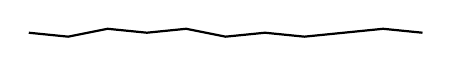
\begin{tikzpicture}
    \draw [thick]
      (0.0,0.15) --
      (0.5,0.10) --
      (1.0,0.20) --
      (1.5,0.15) --
      (2.0,0.20) --
      (2.5,0.10) --
      (3.0,0.15) --
      (3.5,0.10) --
      (4.0,0.15) --
      (4.5,0.20) --
      (5.0,0.15);
  \end{tikzpicture}
  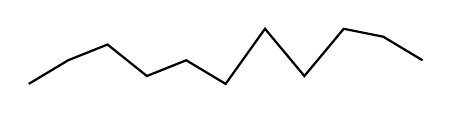
\begin{tikzpicture}
    \draw [thick]
      (0.0,0.1) --
      (0.5,0.4) --
      (1.0,0.6) --
      (1.5,0.2) --
      (2.0,0.4) --
      (2.5,0.1) --
      (3.0,0.8) --
      (3.5,0.2) --
      (4.0,0.8) --
      (4.5,0.7) --
      (5.0,0.4);
  \end{tikzpicture}
  \vspace{0.25cm}
  \caption{Mikrostruktury powierzchni o różnej chropowatości}
	\label{fig:Microstructure}
\end{figure}

Warto zauważyć, że nawet jeżeli wiązka światła odbija się w kierunku
obserwatora nie oznacza to, że wyjdzie z otoczenia powierzchni i trafi do
obserwatora. Mała nierówność może spowodować zasłonięcie obserwatora z
perspektywy tego punktu i odbić się ponownie w zupełnie innym kierunku. Modele
bazujące na mikropowierzchniach zazwyczaj nie biorą pod uwagę odbić
wielokrotnych.

Możliwa jest również sytuacja odwrotna, w której dany punkt może być
teoretycznie zobaczony przez obserwatora, ale światło nie dociera do tego
punktu na skutek przysłaniania źródła światła.

\section{Podstawowe pojęcia radiometryczne}

Rozpocznijmy od podstawowego budulca wiązki światła - fotonu. Energia fotonu
o długości fali $\lambda$ może zostać obliczona korzystając ze wzoru:

$$ Q = \frac{hc}{\lambda} $$

\noindent gdzie $h$ jest stałą Plancka, a $c$ prędkością światła.

Strumień promieniowania (inaczej moc promieniowania, ang. \textit{radiant
flux}) to całkowita ilość energii przechodząca przez określoną powierzchnię w
czasie jednostkowym. Powyższe pojęcie dotyczy wszystkich fal
elektromagmetycznych, zatem jest ono poprawne również dla światła. Jednostką
strumienia promieniowania jest Watt ($\text{W}$).

$$
\Phi = \lim_{\Delta t \rightarrow 0}{
    \frac{\Delta Q}{\Delta t}=\frac{dQ}{dt}
}
$$

Irradiancją nazywamy strumień promieniowania na jednostkę powierzchni:

$$
E(p) =
    \lim_{\Delta \rightarrow 0} {
        \frac{\Delta \Phi(p)}{\Delta A}
    } =
    \frac{d\Phi(p)}{dA}
$$

Oczywiście całkując irradiancję na powierzchni otrzymamy z powrotem strumień
promieniowania:

$$
\Phi = \int_{A} {
    E(p)
    dA
}
$$

W tym miejscu warto zauważyć, że jeżeli powierzchnia $A$ jest nachylona do
strumienia światła $\Phi$ pod pewnym kątem $\alpha$ to irradiancja zmienia się
proporcjonalnie do czynnika $\cos \alpha$. Wynika to z faktu, że obszar na
który padają promienie emitowane przez źródło światła w kierunku prostopadłym
do powierzchni tego źródła jest zależny od kąta pod którym nachylona jest
powierzchnia (rys. \ref{fig:SourceLightAngle}), powierzchnia ta jest odwrotnie
proporcjonalna do czynnika $\cos \alpha$, zatem dzieląc przez powierzchnię
otrzymujemy zależność wprost proporcjonalną dla irradiancji.

\begin{figure}[ht]
  \centering
  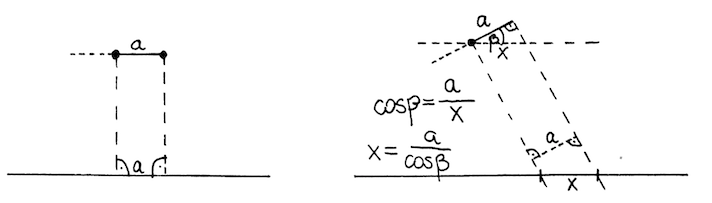
\includegraphics[height=3cm]{pbr/sourcelightangle.png}
  \caption{Wpływ kąta na powierzchnię na które oddziaływuje światło}
  \label{fig:SourceLightAngle}
\end{figure}

W przypadku jednorodnym irradiancję możemy zdefiniować jako średnią moc
promieniowania na pewnej skonczonej powierzchni $A$:

$$
E = \frac{\Phi}{A}
$$

\begin{example}
  Policzmy irradiancję dla światła punktowego w punkcie $p$ na sferze o
  promieniu $r$ o środku w tym właśnie punkcie $p$.

  \[
    E = \frac{\Phi}{4 \pi r^2}
  \]
\end{example}

\textbf{Kątem planarnym} obiektu geometrycznego $G$ z punktu $p$ nazywamy kąt
wyznaczony przez dwie półproste rozpoczynające się w punkcie $p$ wyznaczające
minimalny obszar zawierający obiekt $G$. Miarą kąta planarnego jest
\textit{radian} (\textit{rad}).

% Rysunek kąta geometrycznego
\begin{figure}[ht]
  \centering
  \begin{tikzpicture}
    \coordinate (orig) at (0,0);
    \coordinate (left) at (1,3);
    \coordinate (right) at (5,2);
    \draw (2,1) -- (left) -- (2,4) -- (right) -- (2,1);
    \draw [dashed] (left)--(orig)--(right);
    \draw [fill] (orig) circle [radius=0.08] node [below] {$p$};
    \draw pic[draw=black, <->, "$\theta$", angle eccentricity=1.5] {angle = right--orig--left};
  \end{tikzpicture}
  \caption{Kąt planarny obiektu geometrycznego}
  \label{fig:PlanarAngle}
\end{figure}

\textbf{Kąt bryłowy} jest rozszerzeniem kąta planarnego do trzech wymiarów.
Kątem bryłowym $A$ nazywamy powiechnię rzutu trójwymiarowego obiektu
geometrycznego $G$ na sferę jednostkową o środku w punkcie $p$. Kąt bryłowy
mierzony jest w \textit{steradianach} (\textit{sr}). Kąt bryłowy całej sfery
jednostkowej wynosi $4\pi \:{sr}$.

% Rysunek kąta bryłowego
\begin{figure}[ht]
  \centering
  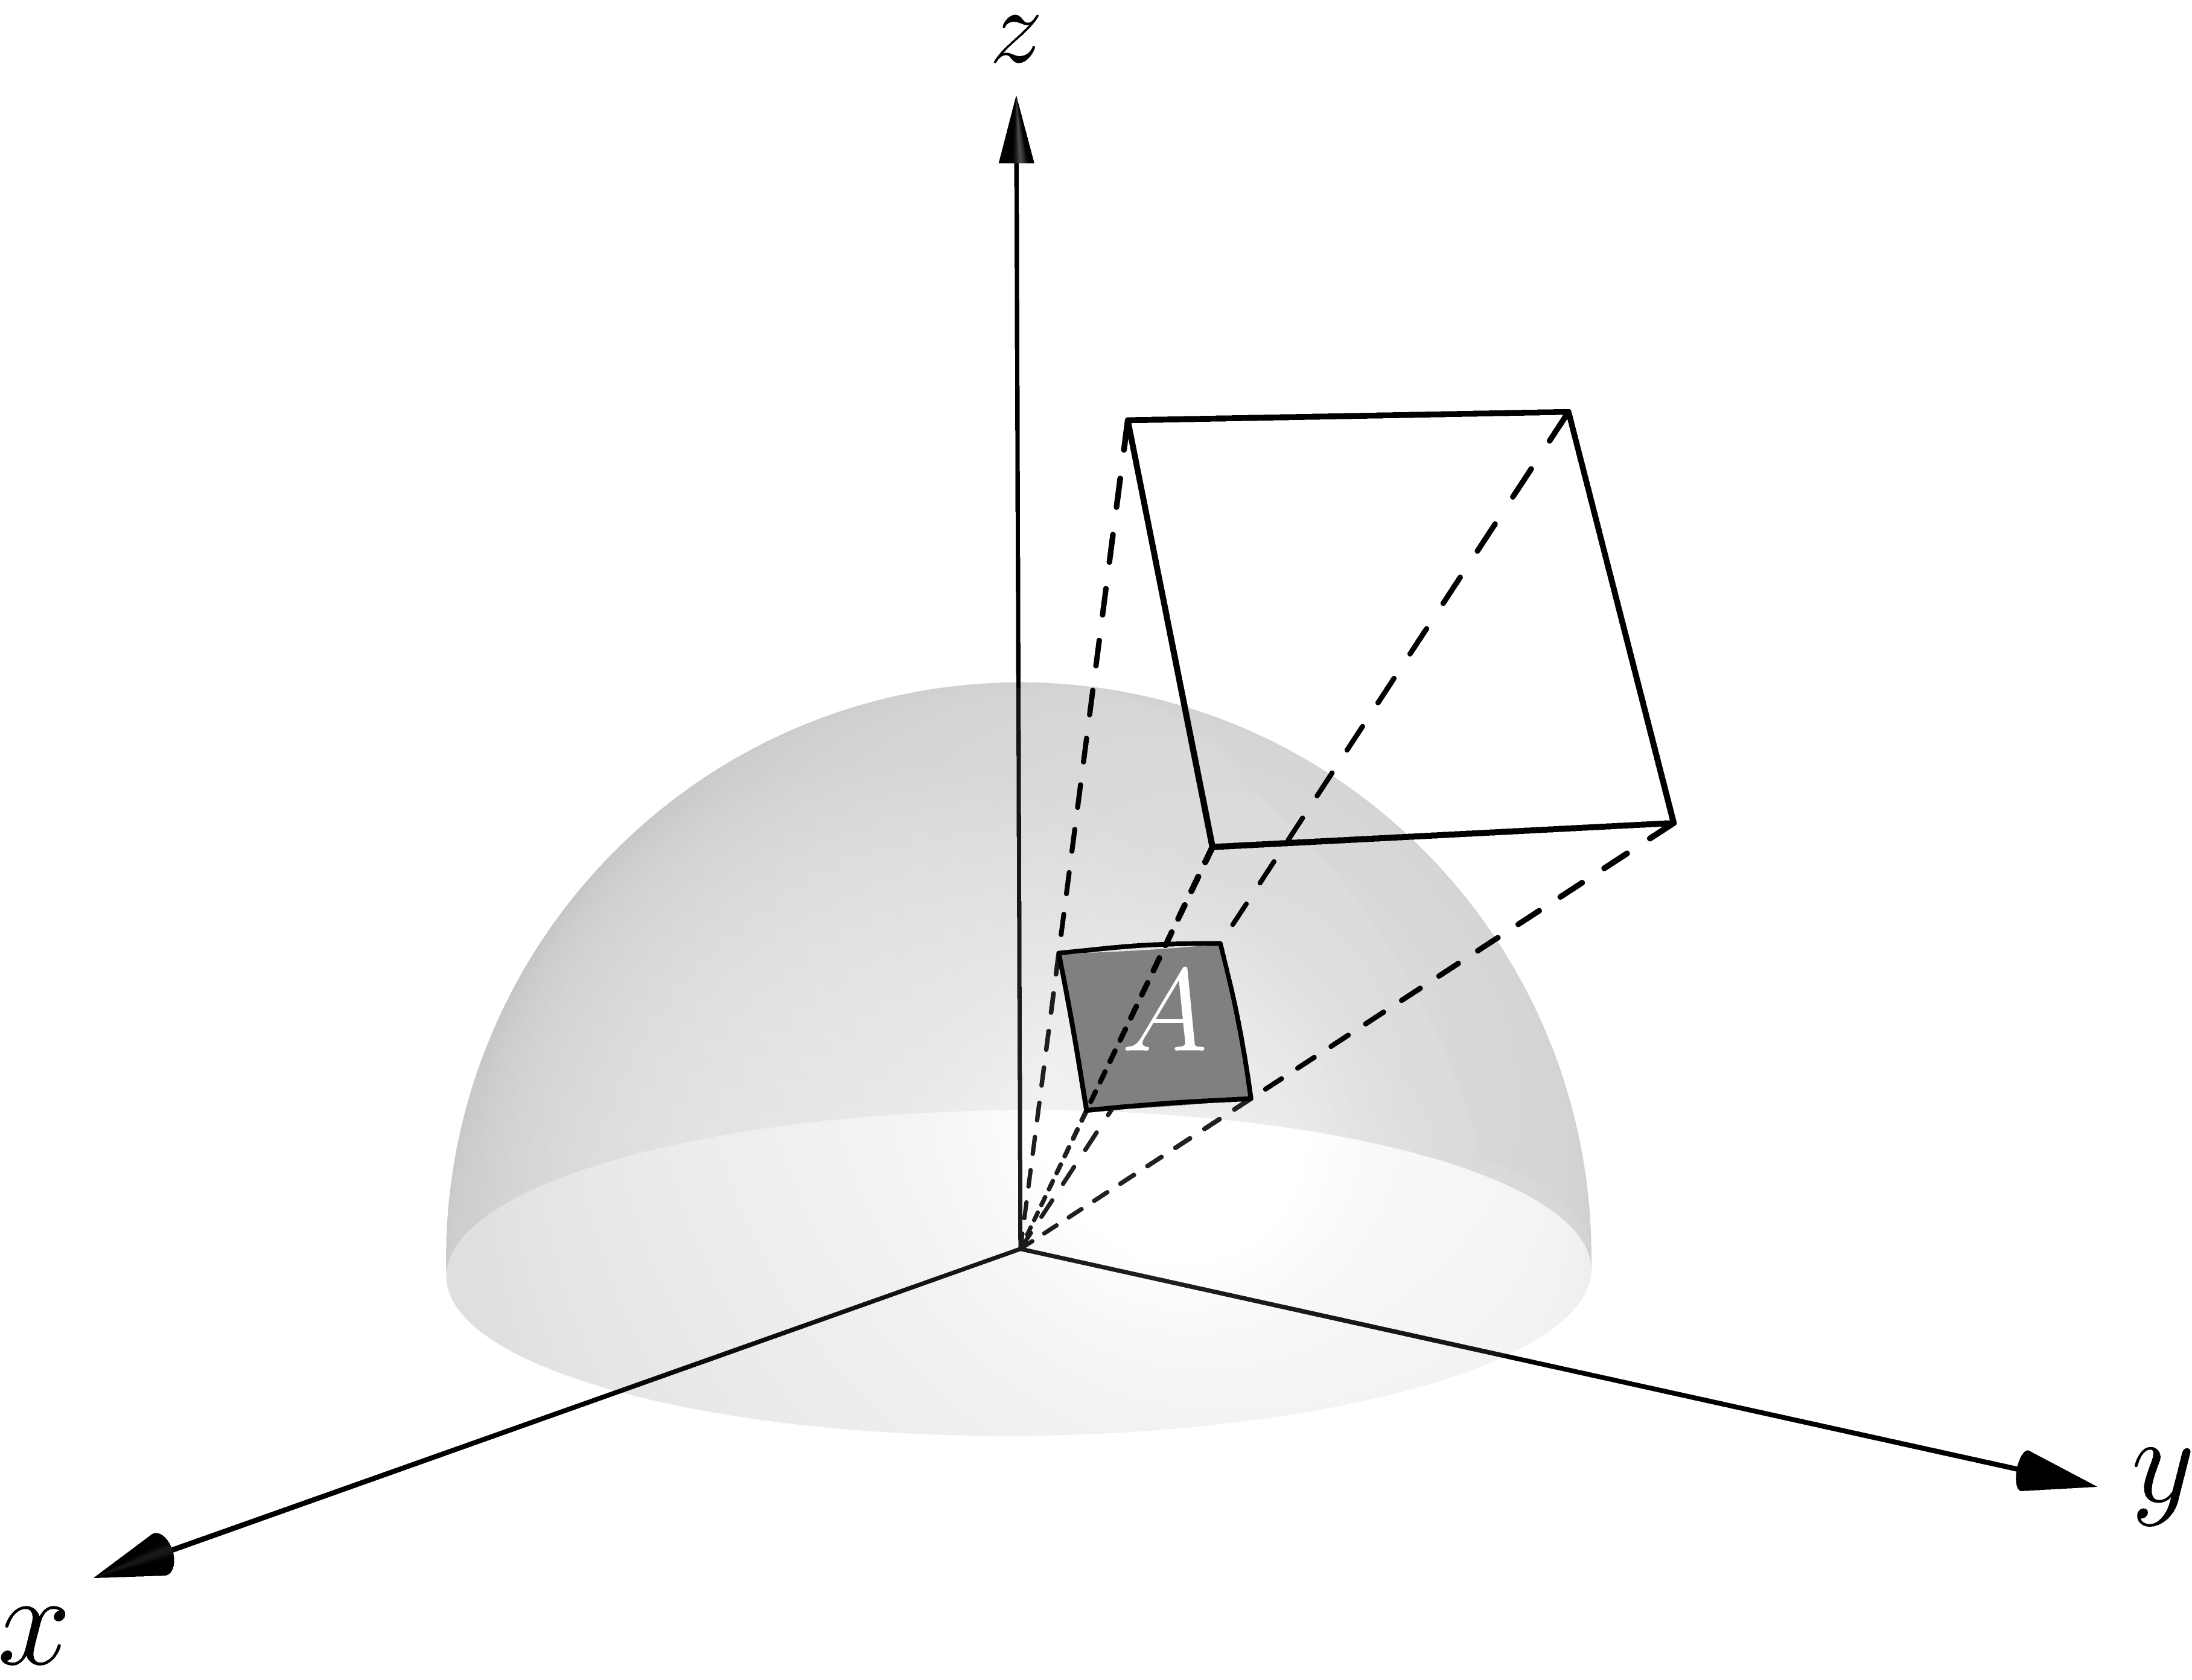
\includegraphics[height=5cm]{pbr/solid_angle.png}
  \caption{Kąt bryłowy powierzchni}
  \label{fig:SolidAngle}
\end{figure}

Kolejną miarą energii jest intensywność. Intensywność jest miarą
rozkładu gęstości mocy światła na kierunkach \cite[p. 328]{pbrt}. Warto na
wstępie zauważyć, że intensywność ma sens tylko i wyłącznie dla teoretycznych
świateł punktowych ze względu na sposób pomiaru kąta. Wartość tą możemy
zdefiniować w następujący sposób:

\begin{gather*}
  I = \lim_{\Delta\omega \rightarrow 0} {
    \frac{\Delta\Phi}{\Delta\omega}
  } = \frac{d\Phi}{d\omega} \\
  \Phi = \int_{\Omega} {I(\omega) d\omega}
\end{gather*}

\noindent gdzie przez $\omega$ rozumiemy wektor określający kierunek ze środka
jednostkowej sfery do punktu leżącego na jej brzegu.

Dla przykładu intensywność jednorodnego światła punktowego wynosi:

\[
  I = \frac{\Phi}{4\pi}
\]

Poprzez $E_{\omega}$ oznaczmy irradiancję hipotetycznej powierzchni
prostopadłej do kierunku $\omega$. Radiancją $L$ nazywamy miarę irradiancji
$E_{\omega}$ w odniesieniu do kąta bryłowego:

$$
L(p, \omega) = \lim_{\Delta\omega \rightarrow 0} {
  \frac{\Delta E_{\omega} (p)}{\Delta\omega}
} =
\frac{d E(p)}{d \omega}
$$

Bardzo ważną obserwacją jest to, że radiancja nie jest mierzona względem
irradiancji powierzchni na której leży punkt $p$, ma to na celu wyeliminowanie
czynnika $\cos \alpha$ z definicji \cite[p. 339]{pbrt}. Jednostką radiancji
jest gęstość energii na jednostkę powierzchni na jednostkę kąta bryłowego.
Radiancję możemy interpretować jako ilość światła wzdłuż jednego promienia.
Radiancja jak i inne miary jest funkcją długości fali.

\section{Równanie renderingu}

\textbf{Równanie renderingu} (ang. \textit{rendering equation}) to równanie
całkowe określające radiancję wychodzącą z danego punktu $p$ w danym kierunku
$\omega_o$ znając radiancję przychodzącą do tego punktu. Równanie te możemy
zapisać jako:

\[
  L_0 =
  L_{e}(p, \omega_o) +
  \int_{\Omega} {
    f_r(p, \omega_i, \omega_o)
    L_i(w_i)
    (n \cdot \omega_i)
    d \omega_i
  }
\]

\noindent gdzie poszczególne składowe to:

\begin{itemize}

  \item $L_e(p, \omega_o$) - całkowita radiancja wyemitowana  w punkcie $p$ w
    kierunku $w_o$

  \item $L_i(\omega_i)$ - radiancja przychodząca z kierunku $\omega_i$

  \item $\Omega$ - jednostkowa półsfera wyznaczająca dziedzinę wszystkich
    możliwych kierunków przychodzących $\omega_i$

  \item $f_{r}(p, \omega_i, \omega_o)$ - funkcja \textit{BRDF} (ang.
    \textit{Bidirectional Reflectance Distribution Function}) wyznaczająca jaka
    część energii przybywającej z kierunku $w_i$ zostanie wysłana w zadanym
    kierunku $w_o$.

\end{itemize}

Aby funkcja BRDF była fizycznie możliwa \todo{Przetłumaczyć Physically
Plausible} musi spełniać dwa warunki. Po pierwsze, funkcja BRDF musi być
niezależna od kolejności parametrów, odwrócenie wszystkich kierunków promieni
powinno dać nam dokładnie ten sam wynik (ang. \textit{reciprocity}):

\[
  \forall_{\omega_i, \omega_o \in \Omega} \quad
  f_r(\omega_i, \omega_o) = f_r(\omega_o, \omega_i)
\]

Po drugie, funkcja BRDF nie może emitować więcej światła niż otrzymuje tzn.:

\[
  \forall_{\omega_i} \quad
  \int_{\Omega} {
    f_r(\omega_i, \omega_o)
    (n \cdot \omega_o)
    d\omega_o
  } \leq 1
\]

Funkcja BRDF zwykle zawiera część refleksyjną oraz część rozproszoną, przez co
większość modeli rozdziela je i analizuje osobno lub definiuje tylko jedną
część. Do podziału najczęściej używane są równania Fresnela.

Istnieje bardzo dużo róznych modeli BRDF \cite{brdf_overview}, my zajmiemy się
natomiast dwoma: najbardziej znanym modelem Blinna-Phonga i modelem
Cooka-Torrance'a.

\subsection{Blinn-Phong BRDF}

Model Blinna-Phonga jest modelem empirycznym, jego równania pochodzą z
obserwacji świata i próby dopasowania prostej funkcji do opisu wielu materiałów
za pomocą małej liczby parametrów.

Podstawowy model Phonga definiował funkcję BRDF w następujący sposób:

\[
f_r(\omega_i, \omega_o) =
  k_d + k_s \left(
    \omega_i \cdot
    \text{reflect}\left(\omega_i\right)
  \right)^{n}
\]

Część rozproszona tego BRDF korzysta ze standardowego modelu Lamberta i
wykorzystuje parametr $k_d$ do określenia koloru materiału \todo{Ten podział
nie do końca jest prawdziwy oraz $k_d$ ze względu na calkę musi być razem z
jakimś współczynnikiem w przypadku bardziej PBR}.

Modyfikacja Blinna polega na wykorzystaniu wektora połówkowego $h$
definiującego teoretyczną powierzchnię która odbiłaby światło z kierunku
$\omega_i$ w kierunku $\omega_o$:

\begin{gather*}
  h = \frac{\omega_i + \omega_o}{||\omega_i+\omega_o||} \\
  f_r(\omega_i, \omega_o) = k_s (n \cdot h)^{n}
\end{gather*}

Co ciekawe, powyższa modyfikacja spowodowała zmniejszenie ilości operacji
wymaganych do obliczenia wyniku, przez co model był wykorzystywany wiele lat
przez domyślne potoki renderowania we wcześniejszych wersjach DirectX oraz
OpenGL. Po podstawieniu do równania renderingu otrzymujemy:

\begin{align*}
  L_0(p, \omega_i, \omega_o) &=
  L_{e}(p, \omega_o) +
  \int_{\Omega} {
    f_r(p, \omega_i, \omega_o)
    L_i(w_i)
    (n \cdot \omega_i)
    d \omega_i
  } = \\
  &= L_{e}(p, \omega_o) +
  k_d \int_{\Omega} {L_i(\omega_i) (n \cdot \omega_i) d\omega_i} +
  k_s \int_{\Omega} {L_i(\omega_i) (n \cdot h)^{n} (n \cdot \omega_i) d\omega_i}
\end{align*}

\subsection{Cook-Torrance BRDF}

Najpopularniejszym \todo{Sprawdić czy są inne znane modele (chyba tak).}
modelem BRDF wykorzystującym podejście mikropowierzchni jest model
Cooka-Torrance'a \cite{CookTorrance}.

Część refleksyjna dla BRDF zdefiniowanego przez Cooka i Torrance'a zapisana
ogólnie wygląda w sposób następujący:

\begin{displaymath}
  f_{\mu} = \frac{
    D(h) F(l,h) G(l,v,h)
  }{
    4 (n \cdot l) (n \cdot v)
  }
\end{displaymath}

Gdzie funkcje $F$, $G$ i $D$ są funkcjami opisującymi zjawiska wspomniane
w rozdziale o analizie interakcji promienia w wiązką światła, są one kolejno:

\begin{itemize}
  \item $D$ - funkcja rozkładu normalnych
  \item $F$ - funkcja Fresnela
  \item $G$ - funkcja geometryczna
\end{itemize}

Funkcja rozkładu normalnych (ang. \textit{Normal Distribution Function, NDF})
opisuje rozkład normalnych mikropowierzchni na pewnej powierzchni o
współczynniku $\alpha$. Konkretniej, funkcja \textit{NDF} $D(h)$ określa
gęstość mikropowierzchni skierowanych w kierunku $h$, które potencjalnie mogą
odbić światło w kierunku obserwatora (chyba, że zostanie przysłonięte lub
całość światła zostanie załamana).

Każda funkcja rozkładu normalnych w postaci znormalizowanej spełnia warunek
\cite{NDFReed}:

\[
  \int_{\omega} {
    D(\omega_i)
    (n \cdot \omega_i)
    d \omega_i
  } = 1
\]

Współczynnik Fresnela opisuje stosunek światła odbitego do światła załamanego
na danej powierzchni pod danym kątem.

Wartość tą opisuje funkcja $F(l,h)$, której wartość będzie odpowiadać
procentowi światła, które zostało odbite. Zatem wartość tego współczynnika musi
znajdować się w przedziale $[0,1]$. Ze względu na złożoność równań Fresnela
koniecznym jest korzystanie z postaci przybliżonej. Popularnymi modelami
opisującymi tą relację są:

\begin{itemize}
\item aproksymacja Schlicka: $F = F_0 + (1 - F_0)(1-V \cdot H)^5$,
\item aproksymacja \textit{Spherical Gaussian} \cite{SphericalGaussianLegarde}:
  $ F = F_0 +(1−F_0) 2^{
    \left(−5.55473\left(V \cdot H\right)−6.98316\right) (V \cdot H)
  } $
\end{itemize}

\begin{figure}[ht]
  \centering
  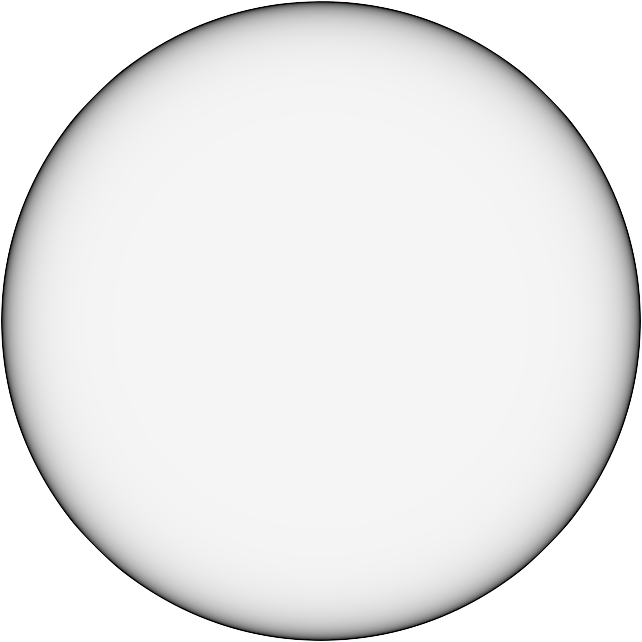
\includegraphics[width=3cm]{pbr/fresnel}
  \caption{Odwrócony współczynnik Fresnela, aproksymacja Schlicka}
\end{figure}

Funckaj geometryczna (lub zaciemnianie geometryczne, ang. \textit{Geometric
Shadowing}) odpowiada za wspomniane wcześniej zjawiska rzucania cieni w obrębie
mikropowierzchni, w związku z czym światło które pada pod pewnym kątem nie
odbija się od całości powierzchni (ang. \textit{shadowing}, rys.
\ref{fig:GeometricShadowing}) oraz zasłaniania promieni odbitych od powierzchni
zmierzających do obserwatora przez inne elementy tej powierzchni w związku z
czym światło odbite nie dociera w całości do obserwatora (ang.
\textit{masking}). W realnym świecie promień po takim zderzeniu nie znika, ale
uproszczone modele traktują takie zachowanie jako absorpcję światła przez
powierzchnię.

Współczynnik związany z zaciemnianiem geometrycznym oznaczymy przez $G(l,v,h)$.
Wartość funkcji $G$ określa nam procent powierzchni skierowanych w kierunku
$h$, które nie są zaciemnione lub zasłonięte.

\begin{figure}[h]
  \centering
  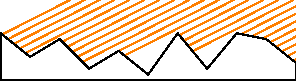
\includegraphics{illustrations/pbr/geometry_shadowing.pdf}
  \vspace{0.25cm}
  \caption{Samozacienianie wewnątrz mikropowierzchni}
  \label{fig:GeometricShadowing}
\end{figure}

Powyższe definicje umożliwają nam zbudowanie ogólnego modelu fizycznego
biorącego pod uwagę podstawowe zjawiska zachodzące w mikropowierzchniach
będących powierzchniami idealnie płaskimi.

\todo[inline]{Dodać część diffuse Cook-Torrance}

\end{document}
